\chapter{深度模型架构}

\section{教育视频关键帧抽取}
    视频中所包含的信息是非常丰富的,但对于教育视频而言,通常冗余、重复的信息占比也很大。
    比如教师上课的一段视频,视频中任意相邻两帧之间的时间差往往在数十毫秒左右,在如此短的时间内,教师几乎无法传达出新的有效信息,从而使得这相邻的两帧所包含的信息几乎完全相同。
    若不加处理地将全量视频信息输入到深度学习模型中进行知识点预测会对计算机造成不必要的负担,同时由于计算量的庞大导致模型迭代收敛的效率低下。
    因此为了减少冗余的信息,同时从教育视频中提取出真正重要且有价值的信息,需要对视频进行关键帧采样。

    教育类视频通常具有增量式\cite{Wang2020FineGrainedSM}的特点,即视频中后一帧的内容可以覆盖前一帧。
    这种增量式的特点也可以用于确定在视频的某一个时刻教师的授课状况:若该时刻的后一帧内容能够覆盖前一帧,说明教师正在延续之前所讲授的知识继续深入;否则说明教师已经讲授完了前面的知识点,现在正在讲授一个新的知识点。
    因此我们可以根据这一特点对教育视频进行关键帧采样,这样每一个关键帧都包含了教师对之前某一个或几个知识点讲解的全部信息。
    同时我们也可以根据这些关键帧对整个视频进行分块,使得每一个知识点的讲解过程都仅处于某一个视频块内,最大限度地保证教育视频信息的局部完整性。
    最后我们使用深度学习模型分别对分割得到的视频块进行知识点预测,综合所有视频块的预测结果得到整个教育视频涉及到的知识点。
    这样不仅能更加充分地利用视频中的所有信息,使得最终预测结果更加可靠,也能让最终的预测结果具有更好的可解释性。

    为此,我们设计了一种类似二分查找的视频关键帧采样算法,伪代码实现如算法 \ref{algo_keyframe} 所示。
    \IncMargin{1em}
    \begin{algorithm}
        \SetKwData{Framep}{$frame_p$}
        \SetKwData{Frameq}{$frame_q$}
        \SetKwData{Framek}{$frame_k$}
        \SetKwData{FPS}{FPS}
        \SetKwData{Video}{Video}
        \SetKwData{Interval}{interval}
        \SetKwData{FrameNum}{frameNum}
        \SetKwData{KeyframeList}{KeyframeList}
        \SetKwData{LowIdx}{lowIdx}
        \SetKwData{HighIdx}{highIdx}
        \SetKwData{MiddleIdx}{middleIdx}
        \SetKwFunction{Min}{min}
        \SetKwFunction{Union}{union}
        \SetKwFunction{CanCover}{canCover}
        \SetKwFunction{SeekFrame}{seekFrame}
        \SetKwInOut{Input}{input}
        \SetKwInOut{Output}{output}

        \Input{Video, FPS, interval, frameNum}
        \Output{List of Keyframes}
        \BlankLine
        % \emph{special treatment of the first line}\;
        \KeyframeList \leftarrow $\emptyset$\;
        \LowIdx \leftarrow $0$\;
        \HighIdx \leftarrow $\Interval \cdot \FPS$\;
        \While{\LowIdx \neq $\FrameNum - 1$}{
            \Framep \leftarrow \SeekFrame{\Video, \LowIdx}\;
            \Frameq \leftarrow \SeekFrame{\Video, \HighIdx}\;
            \If{\CanCover{\Framep, \Frameq}}{
                \LowIdx \leftarrow \HighIdx\;
                \HighIdx \leftarrow \Min{$\FrameNum - 1$, $\LowIdx + \Interval \cdot \FPS$}\;
            }
            \Else{
                \If{\LowIdx == \HighIdx}{
                    \KeyframeList \leftarrow \Union{\KeyframeList, \Framep}\;
                    \LowIdx \leftarrow \HighIdx\;
                    \HighIdx \leftarrow \Min{$\FrameNum - 1$, $\LowIdx + \Interval \cdot \FPS$}\;
                }
                \Else{
                    \MiddleIdx \leftarrow $(\LowIdx + \HighIdx) / 2$\;
                    \Framek \leftarrow \SeekFrame{\Video, \MiddleIdx}\;
                    \If{\CanCover{\Framep, \Framek}}{
                        \LowIdx \leftarrow \MiddleIdx\;
                    }
                    \Else{
                        \HighIdx \leftarrow \MiddleIdx\;
                    }
                }
            }
        }
        \KeyframeList \leftarrow \Union{\KeyframeList, \SeekFrame{\Video, $\FrameNum - 1$}}\;
        \Return{\KeyframeList}\;
        \caption{Keyframe Extraction Algorithm}\label{algo_keyframe}
    \end{algorithm}
    \DecMargin{1em}

    教育类视频经过算法 \ref{algo_keyframe} 处理就可以得到该视频的所有关键帧,每个关键帧都包含了前一段时间内教师所讲授的全部内容。
    整个视频也根据抽取的关键帧分为了多个块,每个视频块以首尾两帧作为关键帧,这段时间内的字幕作为该块视频的对应文本。
    关键帧抽取的结果以及整个模型的架构如图 \ref{fig3.1} 所示。

    \begin{figure}[htb]
        \centering
        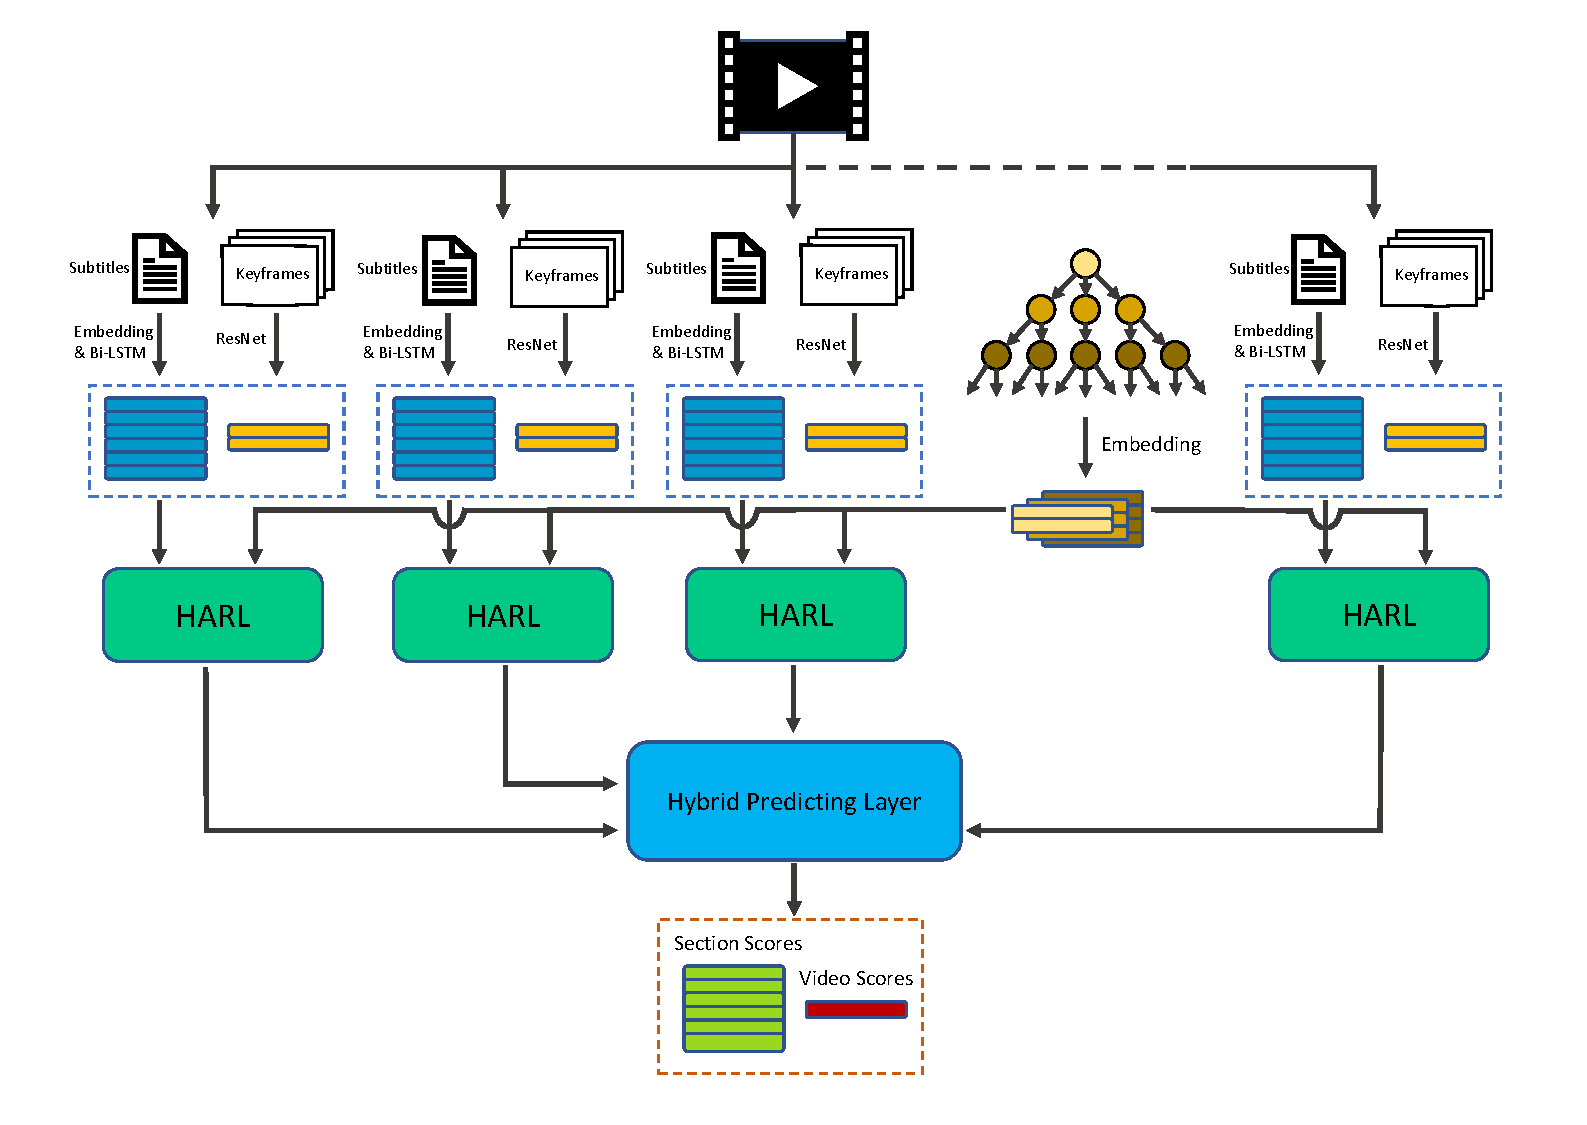
\includegraphics[width=1\linewidth]{model-architect.pdf}
        \caption{深度模型架构}
        \label{fig3.1}
    \end{figure}


\section{多模态特征提取}
    通过关键帧抽取得到了一系列关键帧和相应的视频块与字幕文本,但这些多模态信息并不能直接被计算机理解。
    要利用这些信息进行知识点预测,首先需要通过多模态特征提取将这些多模态信息转化为计算机能够理解并使用的形式。

    对于视频信息,我们可以对每段视频的首尾两帧使用 ResNet\cite{He2016DeepRL} 分别抽取出图像的特征向量,然后将这两个特征向量进行平均,作为该段视频的视频特征。

    对于文本信息而言,文本可以视作为一系列词的组合,因此对文本进行表征本质上就是对词进行表征。
    对于一段包含 $N$ 个词的文本序列 $x = \{w_1, w_2, \dots, w_N\}$,我们使用经过预训练的词向量 GloVe\cite{Pennington2014GloVeGV} 对序列中所有的词进行词嵌入,
    通过将每个词映射为一个固定长度 $d_w$ 的向量,得到表征文本序列的特征向量矩阵 $\boldsymbol{X} = \{v_1, v_2, \dots, v_N\} \in \mathbb{R}^{N \times d_{w}}$。

    同时,知识点体系也可以视为一种模态的信息,类似于我们对文本进行表征的方法,我们也可以将所有的知识点映射为特征向量。
    但这里我们仅用随机向量来表征每个知识点,待模型训练时再对每个知识点的特征向量进行迭代更新和微调。
    至此我们得到了知识点体系的特征矩阵 $\boldsymbol{K} = (K_1, K_2, \dots, K_C) \in \mathbb{R}^{C \times d_c}$,其中 $C$ 为知识点总个数,$d_c$ 为知识点特征向量的长度。
    假设知识点体系共有 $H$ 层,则知识点特征矩阵也可以表示为 $\boldsymbol{K} = [K^1; K^2; \dots; K^H]$。


\section{双向 LSTM}
    我们在多模态特征提取过程中已经将文本序列转化为了词向量特征矩阵,但是这种文本的表征信息密度还不够大。
    在自然语言中,一段文本所包含的信息不仅仅由各个词单独包含的信息堆砌而成,词与词、句与句之间的联系所包含的信息也非常重要,因此我们需要在词向量的基础上进一步抽取出隐含在词与词之间的关联信息。
    我们使用 双向 LSTM\cite{Hochreiter1997LongSM}(双向长短期记忆模型)来对词向量进行进一步的特征提取。
    双向 LSTM 相较于普通的 RNN 而言不仅能获取到文本序列中更长距离的词之间的关联信息,还能同时获取前向和后向的信息。
    输入词向量序列 $\boldsymbol{X} = \{v_1, v_2, \dots, v_N\}$,双向 LSTM 计算隐向量的方式为:
    \begin{equation}
        \begin{aligned}
            &\overrightarrow{h_{n}} = LSTM\left(\overrightarrow{h_{n - 1}}, v_n\right) \\
            &\overleftarrow{h_{n}} = LSTM\left(\overleftarrow{h_{n + 1}}, v_n\right) \\
            &h_n = [\overrightarrow{h_n}, \overleftarrow{h_n}]
        \end{aligned}
    \end{equation}
    其中 $\overrightarrow{h_{n}}$ 为前向传播过程中第 $n$ 个词的隐向量,$\overleftarrow{h_{n}}$ 为后向传播过程中第 $n$ 个词的隐向量,$\overrightarrow{h_{n}}, \overleftarrow{h_{n}} \in \mathbb{R}^{u}$。
    我们将这两个隐向量进行拼接得到隐向量 $h_n \in \mathbb{2u}$,即为文本序列中第 $n$ 个词连同其上下文信息的特征向量。
    因此词向量特征矩阵经过 双向 LSTM 后得到的输出为 $V = (h_1, h_2, \dots, h_N) \in \mathbb{R}^{N \times 2u}$。
    此外,我们在词的维度对隐向量矩阵取平均,将 $N$ 个词的所有信息融合到一个特征向量中,得到文本序列的一个统一特征表示向量 $\tilde{V} = avg(V) = avg(h_1, h_2, \dots, h_N)$


\section{基于注意力的循环网络}
    在提取出视频、文本、知识点体系等多模态信息的特征向量之后,我们将使用基于注意力机制的循环神经网络 HARL\cite{Huang2019HierarchicalMT} 对输入每块视频的多模态信息进行整合和知识点预测。
    HARL 是一个基于循环与注意力的模型,能够对层级知识点体系自上而下地逐层预测知识点。
    基于注意力的记忆单元 HAM 是 HARL 网络的基本单元,每一个 HAM 都是层级知识点体系中的某一层知识点的预测单元,多个 HAM 串联起来就构成了具有循环结构的 HARL。
    HAM 原本是用于使用注意力机制捕获文本与知识点之间的关联,但只要我们对 HAM 内部实现稍作修改就可以用于捕获视频与文本、标签与文本等多模态信息之间的关联关系。
    除此之外,在对第 $h$ 层知识点进行预测时,HAM 能够整合第 $h - 1$ 层已经预测的知识点的信息来指导本层知识点的预测,同时生成指导第 $h + 1$ 层进行知识点预测的语义信息。
    考虑到层级知识点体系从上到下通常伴随着知识点的逐渐细化与具体,HARL 自上而下的预测方式也具有现实意义与合理性。
    HARL 网络的整体架构和 HAM 的内部实现如图 \ref{fig3.2} 所示。

    \begin{figure}[htb]
        \centering
        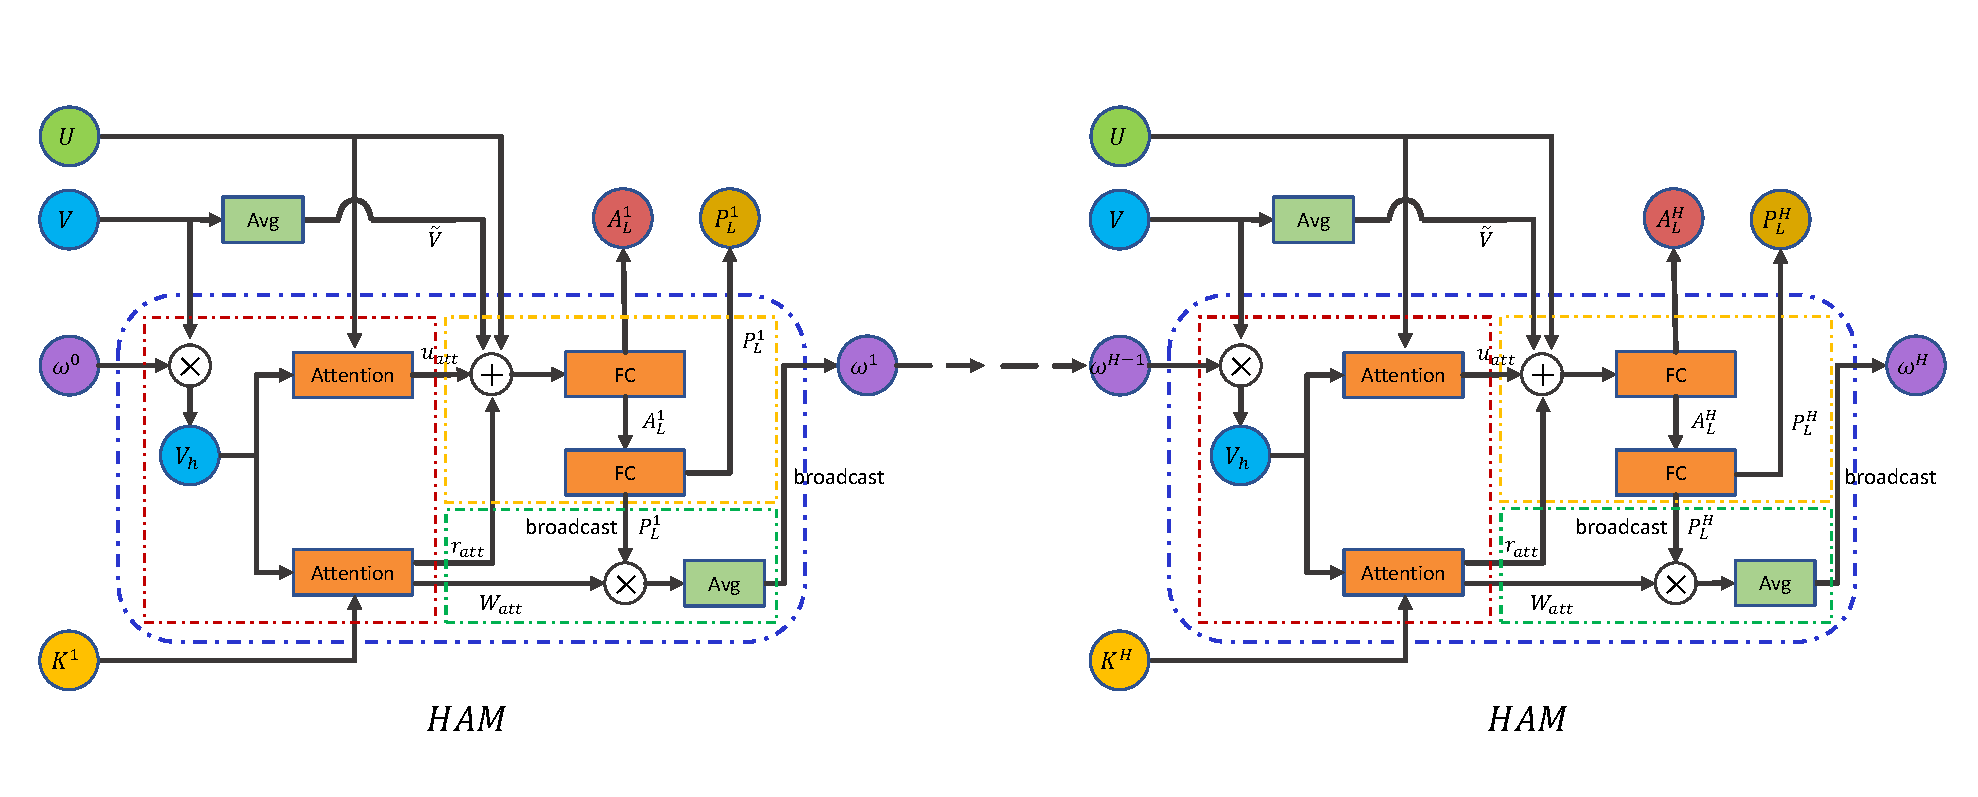
\includegraphics[width=1\linewidth]{HARL.pdf}
        \caption{HARL}
        \label{fig3.2}
    \end{figure}

\subsection{基于注意力的记忆单元}
    HAM 主要包含三个模块,VTKA 模块、KPM 模块以及 KDM 模块。

    其中 VTKA 模块为 Video-Text-Knowledge Attention,即视频-文本-知识点注意力模块,该模块接收视频、文本、当前层知识点表征以及来自上一层 HAM 的知识点预测语义信息,
    从而结合这四个方面的信息捕捉视频、文本与当前层知识点之间的关联信息。
    KPM 模块为 Knowledge Prediction Module,即知识点预测模块,该模块主要用于接受来自 VTKA 模块捕捉到的关联信息,结合初始的视频、文本表征对当前层的知识点进行预测。
    同时生成一个包含了视频、文本、当前层知识点信息的统一特征表示。
    KDM 模块为 Knowledge Dependency Module,即知识点依赖模块。该模块接受来自 VTKA 的关联信息和 KPM 对当前层知识点的预测结果,根据这两个计算结果来获取不同层知识点之间的依赖关系。
    该依赖关系将被送到下一层 HAM 中对下一层知识点的预测提供指导信息。

    因此对第 $h$ 层的 HAM,输入视频特征向量 $\boldsymbol{U}$,文本特征向量矩阵 $\boldsymbol{V}$,来自上一层的知识点依赖信息 $\omega^{h - 1}$ 以及知识点特征向量 $K^h$,各模块输出的计算公式为:
    \begin{equation}
        \begin{aligned}
            &\tilde{V} = avg(\boldsymbol{V}) \\
            &r_{att}^h, W_{att}^h, u_{att}^h = VTKA(\boldsymbol{\omega^{h - 1}}, U, \boldsymbol{V}, \boldsymbol{K^h}) \\
            &P_L^h, A_L^h = KPM(\tilde{V} \oplus U \oplus r_{att}^h \oplus u_{att}^h) \\
            &\boldsymbol{\omega^h} = KDM(W_{att}, P_L^h)
        \end{aligned}
    \end{equation}
    其中,$r_{att}^{h}, W_{att}^h$ 分别为包含了文本-知识点关联信息的特征向量和注意力矩阵,$u_{att}^h$ 为包含了视频-文本关联信息的特征向量,
    $P_L^h, A_L^h$ 分别为 HAM 对当前层知识点的预测结果和对当前层输入的统一表示,$\boldsymbol{\omega^h}$ 则代表了第 $h$ 层知识点依赖关系的融合信息,
    特别地,我们将 $\boldsymbol{\omega^0}$ 初始化为一个全 $1$ 矩阵,表示在得知层级知识点体系的第一层的有关信息之前没有任何先验知识。

    下面我们对 HAM 的三个模块结构进行详细说明。

    \subsubsection{VTKA}
    视频-文本-知识点注意力模块旨在使用注意力机制对多模态信息进行特征融合,并获取其中的关联信息。
    对于第 $h$ 层 HAM,首先我们将来自上一个 HAM 的知识点依赖信息 $\boldsymbol{\omega^{h - 1}} \in \mathbb{R}^{N \times 2u}$ 注入到文本信息中:
    \begin{equation}
        \boldsymbol{V}_h = \boldsymbol{\omega^{h - 1}} \otimes \boldsymbol{V}
    \end{equation}
    这里 $\otimes$ 代表矩阵逐项相乘的操作,运算结果 $\boldsymbol{V}_h \in \mathbb{R}^{N \times 2u}$ 就是融合了文本信息和已知的知识点层级依赖信息的结果。

    考虑到一个视频的不同片段、与之对应的文本的不同部分可能涉及到不同的知识点,我们使用注意力机制来捕获文本信息和知识点之间更细粒度的关系,计算方式如下:
    \begin{equation}
        \begin{aligned}
            &O_h = tanh(\boldsymbol{W}_s^h \cdot \boldsymbol{V}_h^T) \\
            &W_{att}^h = softmax(K^h \cdot O_h)
        \end{aligned}
    \end{equation}
    其中 $\boldsymbol{W}_s^h$ 是一个随机初始化的、可训练的参数矩阵。计算 $O_h$ 的目的在于改变 $V_h$ 的维度,使其能够与 $K^h$ 进行矩阵运算,从而计算注意力矩阵。
    $W_{att}^h \in \mathbb{R}^{\left|K^h\right| \times N}$ 即为文本信息与当前层知识点信息之间的注意力矩阵,包含了二者的关联信息。
    记 $W_{att}^h = (W_1^h, W_2^h, \dots, W_{\left|K^h\right|}^h)$,经过 $softmax$ 操作后 $W_{att}^h$ 的每一个行向量 $W_i^h \in \mathbb{R}^N$ 之和都为 1。
    $W_i^h$ 中的注意力分数都可以视为权重值,这代表着文本信息中的不同部分与知识点 $i$ 的关联相似程度。
    因此可以使用该注意力分数矩阵来对多模态信息进行加权平均:
    \begin{equation}
        M_h = W_{att} \cdot \boldsymbol{V}_h
    \end{equation}
    从而得到融合了第 $h$ 层知识点标签信息的文本信息特征矩阵 $M_h \in \mathbb{R}^{{\left|K^h\right|} \times 2u}$,
    $M_h$ 中每一个行向量 $M_i$ 都是文本信息在受到第 $i$ 个知识点影响后的特征向量。
    接着我们再对 $M_h$ 做平均池化,可以得到具有当前第 $h$ 层所有知识点信息的特征向量 $r_{att}^h \in \mathbb{R}^{2u}$:
    \begin{equation}
        r_{att}^h = avg(M_h)
    \end{equation}

    同样的,考虑到视频关键帧与对应文本段的不同部分关联程度可能不同,类似于上面的步骤,我们也通过注意力机制来捕获文本段与视频关键帧之间的关联关系:
    \begin{equation}
        \begin{aligned}
            &O_h' = tanh(\boldsymbol{W}_u^h \cdot \boldsymbol{V}_h^T) \\
            &w^h = softmax(\boldsymbol{U} \cdot O_h') \\
            &u_{att}^h = w^h \cdot \boldsymbol{V}_h
        \end{aligned}
    \end{equation}
    其中 $\boldsymbol{W}_s^h$ 也是一个随机初始化的、可训练的参数矩阵。最终得到的特征向量 $u_{att}^h$ 为 $\boldsymbol{V}_h^T$ 的词向量加权平均而来,
    与视频特征向量 $\boldsymbol{U}$ 关联相似程度越高的词向量,其信息在 $u_{att}^h$ 中的保留程度也就越高。

    \subsubsection{KPM}
    在 VTKA 提取出多模态信息与知识点信息的关联关系之后,KPM 模块将结合特征向量 $r_{att}^h$ 和原始的视频、文本特征 $\boldsymbol{U}, \boldsymbol{\tilde{V}}$ 生成包含第 $h$ 层所有信息的统一特征向量 $A_L^h$,
    同时使用该特征向量对当前层的知识点进行预测,得到当前第 $h$ 层的所有知识点预测分数 $P_L^h$。具体计算公式如下:
    \begin{equation}
        \begin{aligned}
        &A_L^h = \varphi\left(W_T^h \cdot \left[U \oplus \tilde{V} \oplus r_{att}^h\right] + b_T^h\right) \\
        &P_L^h = \sigma\left(W_L^h \cdot A_L^h + b_L^h\right)
        \end{aligned}
    \end{equation}
    其中,$\varphi$ 为非线性激活函数 $ReLU$,$\sigma$ 为 $sigmoid$ 激活函数,用于将预测分数归一化。
    $W_T^h \in \mathbb{R}^{v \times (4u + d_v)}, W_L^h \in \mathbb{R}^{{\left|K^h\right|} \times v}$ 为随机初始化的、可训练的参数矩阵,
    $b_T^h \in \mathbb{R}^{v}, b_L^h \in \mathbb{R}^{\left|K^h\right|}$ 为随机初始化的、可训练的偏置向量。

    \subsubsection{KDM}
    KDM 模块主要用于捕捉当前层知识点体系的特征,通过将结果输出到下一层 HAM 中参与运算,从而达到对层级知识点体系不同层之间的关联进行建模的目的。
    对于第 $h$ 层中的知识点,考虑到不同的知识点对预测结果有着不同的信息贡献,我们将使用第 $h$ 层的预测结果 $P_L^h$ 来对 VTKA 模块输出的注意力矩阵 $W_{att}^h$ 进行进一步的调整。
    以 $P_L^h$ 预测分数为权重,通过逐项相乘的方式来对 $W_{att}^h$ 中的信息作出取舍:
    \begin{equation}
        E^h = broadcast(P_L^h) \otimes W_{att}^h
    \end{equation}
    其中,$broadcast$ 操作意在将向量 $P_L^h$ 转变为与 $W_{att}^h$ 具有相同维度的矩阵,以便后续的矩阵操作,
    即 $broadcast(P_L^h) = \left((P_L^h)^T, (P_L^h)^T, \dots, (P_L^h)^T\right) \in \mathbb{R}^{\left|K^h\right| \times N}$。
    注意到 $P_L^h$ 中的每一个预测分数值都在 $0 \sim 1$ 之间,因此逐项相乘操作的意义在于根据预测值来决定每个知识点保留的信息量。
    对于预测值较大的知识点,说明该知识点与输入的多模态信息关联性更强,逐项相乘也将会保留更多的有关该知识点的信息,反之亦然。
    因此 $E^h = (e_1^h, e_2^h, \dots, e_{\left|K^h\right|}^h) \in \mathbb{R}^{\left|K^h\right| \times N}$ 即为注意力矩阵 $W_{att}^h$ 经过信息取舍之后的结果。

    接着,我们继续对 $E^h$ 做平均池化操作,将所有 $\left|K^h\right|$ 个标签的信息融入到一个向量表征 $\tilde{E^h} \in \mathbb{R}^{N}$ 中:
    \begin{equation}
        \tilde{E^h} = avg(E^h)
    \end{equation}

    最后,我们再对 $\tilde{E^h}$ 做 $broadcast$ 操作,得到向下一层 HAM 传递的知识点依赖关系矩阵 $\boldsymbol{\omega}^h$:
    \begin{equation}
        \boldsymbol{\omega}^h = broadcast(\tilde{E}^h)
    \end{equation}
    其中 $\boldsymbol{\omega}^h = (\omega_1^h, \omega_2^h, \dots, \omega_N^h) \in \mathbb{R}^{N \times 2u}$ 包含了多模态输入与第 $h$ 层所有知识点的关联信息,
    以及第 $h$ 层知识点本身的信息。将该矩阵传入到下一层 HAM 中参与计算也是对真实情况中上层知识点影响下层知识点这一特点的建模。


\section{混合预测模块}
    将多模态信息输入 HARL 模型之后,我们可以得到每一层知识点的预测结果 $P_L^h$,以及包含了每一层的知识点信息与多模态输入信息的统一表征向量 $A_L^h$。
    从 HARL 中得到的逐层的知识点预测结果是对层级知识点体系局部预测的集合,而在层级多标签预测任务中,对整个层级结构进行全局的预测也非常重要。
    因此我们将对所有层的统一特征向量进行信息综合,然后进行对所有知识点的全局预测。

    记 $A_L = (A_L^1, A_L^2, \dots, A_L^H) \in \mathbb{R}^{H \times v}$ 为所有局部统一表征向量构成的特征矩阵,
    我们对该矩阵做平均池化操作,将 $H$ 层的特征向量进行综合,得到特征向量 $\tilde{A_L}$:
    \begin{equation}
        \tilde{A}_L = avg(A_L)
    \end{equation}
    然后再通过 MLP 得到全局的特征向量 $A_G$ 和全局的知识点预测结果 $P_G$:
    \begin{equation}
        \begin{aligned}
            A_G = \varphi\left(W_G \cdot \tilde{A}_L + b_G\right)
            P_G = \sigma\left(W_M \cdot A_G + b_M\right)
        \end{aligned}
    \end{equation}
    其中 $W_G \in \mathbb{R}^{v \times v}, W_M \in \mathbb{R}^{C \times v}$ 为随机初始化的、可训练的参数矩阵,
    $b_G \in \mathbb{R}^{v}, b_M \in \mathbb{R}^{C}$ 为随机初始化的、可训练的偏置向量,
    $\varphi$ 为非线性激活函数 $ReLU$,$\sigma$ 为 $sigmoid$ 激活函数,用于将预测分数归一化。
    $P_G$ 中每个预测分数的值都在 $0 \sim 1$ 之间,表示预测为对应知识点的概率值。

    我们记 $P_L = \left(P_L^1 \oplus P_L^2 \oplus \cdots \oplus P_L^H\right) \in \mathbb{R}^{C}$,
    将所有知识点层级的局部预测结果包含到一个向量 $P_L$ 中,其中 $\oplus$ 为向量的拼接操作。
    为了将局部预测与全局预测进行综合,我们使用加权平均的方式得到最终的知识点预测分数 $P_F \in \mathbb{R}^{C}$:
    \begin{equation}
        P_F = (1 - \alpha) \cdot P_L + \alpha \cdot P_G
    \end{equation}
    其中 $\alpha \in [0, 1]$ 为可改变的权重超参,用于确定在最终知识点预测分数中全局预测分数的占比,
    $\alpha = 1$ 表示只考虑全局的预测结果而忽略逐层的、局部的预测结果。

    至此,我们完成了对一个视频块的知识点预测,要预测整个教育视频所涉及的知识点,还需要将所有视频块的特征向量和预测结果进行综合。
    若该视频在关键帧抽取阶段被分割为 $S$ 段,则我们记 $A_{L_i} = \left(A_{L_i}^1, A_{L_i}^2, \dots, A_{L_i}^H\right)$ 为第 $i$ 个视频块的所有局部统一表征向量构成的特征矩阵,
    则整个视频的特征向量矩阵为 $A_{LV} = \left(A_{L_1}, A_{L_2}, \dots, A_{L_S}\right) \in \mathbb{R}^{S \times H \times v}$。
    类似于对某个单独的视频块所做的全局预测分数计算,我们也可以用相同的方式通过 $A_{LV}$ 计算出整个视频的全局预测分数 $P_{GV} \in \mathbb{R}^{C}$:
    \begin{equation}
        \begin{aligned}
            &\tilde{A}_{LV} = avg\left(A_{L_1}, A_{L_2}, \dots, A_{L_S}\right) \\
            &A_{GV} = \varphi\left(W_{GV} \cdot \tilde{A}_{LV} + b_{GV}\right) \\
            &P_{GV} = \sigma\left(W_{MV} \cdot \tilde{A}_{GV} + b_{MV}\right)
        \end{aligned}
    \end{equation}
    其中 $W_{GV} \in \mathbb{R}^{v \times v}, W_{MV} \in \mathbb{R}^{C \times v}$ 为随机初始化的、可训练的参数矩阵,
    $b_{GV} \in \mathbb{R}^{v}, b_{MV} \in \mathbb{R}^{C}$ 为随机初始化的、可训练的偏置向量。

    同样类似于对某个单独的视频块所作的最终预测分数计算,我们也期望使用整个视频的局部和全局预测分数来进行加权平均,得到最终预测分数。
    记 $P_{L_i} = \left(P_{L_i}^1 \oplus P_{L_i}^2 \oplus \cdots \oplus P_{L_i}^H\right)$ 为第 $i$ 个视频块的局部预测结果,则将所有视频块分别经过 HARL 模型预测之后,
    我们可以得到整个视频的局部预测分数矩阵 $P_{LV} = \left(P_{L_1}, P_{L_2}, \dots, P_{L_S}\right)$。
    类似地,我们通过对 $P_{LV}$ 做最大池化操作,将所有视频块的局部预测分数进行综合,可以得到表示整个视频局部预测分数的向量 $\tilde{P}_{LV} \in \mathbb{R}^{C}$,即:
    \begin{equation}
        \tilde{P}_{LV} = max\left(P_{L_1}, P_{L_2}, \dots, P_{L_S}\right)
    \end{equation}
    最终,通过对 $P_{LV}$ 和 $P_{GV}$ 进行加权平均,得到整个视频的最终预测分数 $P_{FV} \in \mathbb{R}^{C}$:
    \begin{equation}
        P_{FV} = (1 - \alpha) \cdot P_{LV} + \alpha \cdot P_{GV}
    \end{equation}
    其中参数 $\alpha$ 与计算某个视频块所用的参数 $\alpha$ 相同。


\section{损失函数}
    考虑到在混合预测模块中我们通过对局部与全局预测分数进行加权平均得到最终的预测分数,在损失函数中我们也应当分别考虑真实知识点标签和局部、全局预测分数之间的差异。
    同时,来自同一个视频的所有视频块应当满足一致性,即任何一个单独视频块的预测知识点集合应当为整个视频的真实知识点集合的子集。

    为了对以上两种关系进行建模,我们设计了以下的损失函数:
    \begin{equation}
        \begin{aligned}
            &\mathcal{L}_L = \varepsilon\left(\tilde{P}_{LV}, \left(Y_L^1 \oplus Y_L^2 \oplus \cdots \oplus Y_L^H\right)\right) \\
            &\mathcal{L}_G = \varepsilon\left(P_{GV}, Y_G\right) \\
            &\mathcal{L}_C = \varepsilon\left(max\left(P_{F_1}, P_{F_2}, \dots, P_{F_S}\right), Y_G\right)
        \end{aligned}
    \end{equation}
    其中,$\varepsilon$ 为交叉熵损失函数,$Y_L^h$ 为位于第 $h$ 层的真实标签,$Y_G$ 为所有的真实知识点标签,$P_{F_i}$ 则为第 $i$ 个视频块的最终预测分数。

    以上三个损失函数的含义分别为:$\mathcal{L}_L$ 用于衡量视频局部预测分数与真实知识点标签之间的区别,$\mathcal{L}_G$ 用于衡量全局预测分数与真实知识点标签之间的区别。
    $\mathcal{L}_C$ 是对视频块与视频之间一致性进行建模的损失,衡量所有视频块的预测知识点集合的合集与真实知识点标签之间的差异。

    因此我们最终的损失函数 $\mathcal{L}$ 为:
    % \begin{equation}
    %     \mathcal{L} = \mathcal{L}_L + \mathcal{L}_G + \mathcal{L}_C + \lambda\lVert\Theta\rVert
    % \end{equation}
    % 其中 $\Theta$ 代表模型中所有的可训练参数,$\lambda$ 为可调整的正则化系数,这一部分主要用于限制模型的复杂度,防止模型训练时可能出现的过拟合。

    \begin{equation}
        \mathcal{L} = \mathcal{L}_L + \mathcal{L}_G + \mathcal{L}_C
    \end{equation}

    最后,我们使用 Adam\cite{Kingma2015AdamAM} 优化器来降低损失 $\mathcal{L}$,从而达到对模型参数迭代更新和优化的目的。
